\documentclass[12pt]{article}


%%%%%%%%%%%%%%%%%%%%%%%%%%%%%%%%%%%%%%%%%%%%
%% Page formatting.
%%%%%%%%%%%%%%%%%%%%%%%%%%%%%%%%%%%%%%%%%%%%%%
\usepackage[margin=1in]{geometry} % adjust margins
\setlength\parindent{0em} % never indent a paragraph
\setlength{\parskip}{1em} %Seperate paragraphs


%%%%%%%%%%%%%%%%%%%%%%%%%%%%%%%%%%%%%%%%%%%%
%% Packages
%%%%%%%%%%%%%%%%%%%%%%%%%%%%%%%%%%%%%%%%%%%%%%
\usepackage{amsthm, amssymb, amsmath, relsize}
\usepackage[colorlinks=true, allcolors=blue]{hyperref} 
\usepackage{enumerate}  
\usepackage{mathrsfs}
\usepackage{xcolor}
\usepackage{tikz} % for making graphs and drawings
\usetikzlibrary{arrows.meta}

%%%%%%%%%%%%%%%%%%%%%%%%%%%%%%%%%%%%%%%%%%%%%%
%% Add any additional packages below.
%%%%%%%%%%%%%%%%%%%%%%%%%%%%%%%%%%%%%%%%%%%%%%


%%%%%%%%%%%%%%%%%%%%%%%%%%%%%%%%%%%%%%%%%%%%%%



%%%%%%%%%%%%%%%%%%%%%%%%%%%%%%%%%%%%%%%%%%%%%%
%% Auto-Counter for homework problems
%%%%%%%%%%%%%%%%%%%%%%%%%%%%%%%%%%%%%%%%%%%%%%
\newcounter{HWcounter}
\setcounter{HWcounter}{1}
\newcommand{\problem}{\textbf{Problem  \theHWcounter.} \addtocounter{HWcounter}{1}}
\newcommand{\answer}{\vspace{2em} \textbf{Solution. }}
%%%%%%%%%%%%%%%%%%%%%%%%%%%%%%%%%%%%%%%%%%%%%%



%%%%%%%%%%%%%%%%%%%%%%%%%%%%%%%%%%%%%%%%%%%%
%% Define (or redefine) any commands/macros here
%%%%%%%%%%%%%%%%%%%%%%%%%%%%%%%%%%%%%%%%%%%%%%
\newcommand{\R}{\mathbb{R}} % sets up the command \R to write the R symbol for real numbers
\newcommand{\Z}{\mathbb{Z}} % use \Z for integers
\newcommand{\Q}{\mathbb{Q}} % use \Q for rationals
\newcommand{\N}{\mathbb{N}} % use \N for natural numbers

\definecolor{mypink2}{HTML}{F67599}
\definecolor{mypink}{HTML}{F8A3BC}
\definecolor{mypurple}{HTML}{EEDAEA}
\definecolor{mygreen}{HTML}{D9EA9A}
\definecolor{myblue}{HTML}{A4DBE8}
\definecolor{myyellow}{HTML}{FBDD7A}



%%%%%%%%%%%%%%%%%%%%%%%%%%%%%%%%%%%%%%%%%%%%



\begin{document}


% This establishes the title and author.
\title{Homework 3}
\author{Harry Chen}
\date{Due: February 6, 2026} % delete this line if you want to automatically insert the date
\maketitle





\problem Prove the geometric partial sum formula for constant $r$ and $|r|<1$, ie prove 
\[ \sum_{n=0}^k r^n = \dfrac{1 - r^{k+1}}{1-r} \]

\answer  %%%% ANSWER TO PROBLEM 1 HERE %%%%
\\
For this problem, we prove by Induction. 
\\
%\vspace*{2cm} 用作段落换行
\\
\textbf{Base Case: } It is evident that when $ k_0=0$,  
\[ LHS = \sum_{n=0}^0 r^n = 1 = \dfrac{1 - r}{1-r}  \]
satisfied.\\
\\
\textbf{Inductive Step: }
Assume that for some $k=k_0\in \N$,
\[
\sum_{n=0}^{k_0} r^n = \frac{1 - r^{k_0+1}}{1 - r}.
\]
We need to prove that for $k=k_0+1$, the statement of
\[
\sum_{n=0}^{k_0+1} r^n = \frac{1 - r^{(k_0+1)+1}}{1 - r}.
\]
is also satisfied.
\\
\vspace*{2cm}
\\
To prove this, we start from the left-hand side,
\begin{align}
LHS = \sum_{n=0}^{k_+1} r^n
&= \sum_{n=0}^{k_0} r^n + r^{k_0+1} \\
\end{align}
By using the result for $k=k_0$, we have,
\begin{align}
LHS 
&= \frac{1 - r^{k_0+1}}{1 - r} + r^{k_0+1} \\
&= \frac{1 - r^{k_0+1} + r^{k_0+1}(1 - r)}{1 - r} \\
&= \frac{1 - r^{k_0+2}}{1 - r}\\
&= \frac{1 - r^{(k_0+1)+1}}{1 - r}\\
&=RHS
\end{align}
\\
\\
Thus, by mathematical induction, 
\[ \sum_{n=0}^k r^n = \dfrac{1 - r^{k+1}}{1-r} \]
is true for all $n \in \N$.
\qed









\newpage
\problem Prove that for sets $A$ and $B$: 
\[ \mathscr{P}(A \setminus B) \setminus \{\emptyset\} \subseteq \mathscr{P}(A) \setminus \mathscr{P}(B) . \]
\answer  %%%% ANSWER TO PROBLEM 2 HERE %%%%
\\
Let $X$ an arbitrary element $X\in \mathscr{P}(A \setminus B) \setminus \{\emptyset\}$, then element $X \neq \emptyset$, and element $X\in \mathscr{P}(A \setminus B)$. By the definition of a power set, $X\subseteq A \setminus B $. Therefore, $\forall x \in X$, $x$ is in $A$ but $x$ is not in B. Since this holds for all $x \in X$, we conclude that
\[ X \subseteq A \]
By the definition of power set 
\[X\in  \mathscr{P}(A)\]
Moreover,
\[ X \cap B = \emptyset \]
Since $X \neq \emptyset$, $X \notin \mathscr{P}(B)$.\\
By the definition of set minus, 
\[ X \in \mathscr{P}(A) \setminus \mathscr{P}(B)\]
Hence, 
\[ \mathscr{P}(A \setminus B) \setminus \{\emptyset\} \subseteq \mathscr{P}(A) \setminus \mathscr{P}(B) . \]





\newpage
\problem Let $A,B,C$ be nonempty sets. Prove that if $A \times C = B \times C$, then $A = B$.

\answer\\  %%%% ANSWER TO PROBLEM 3 HERE %%%%
\\
For this problem, prove by using contraposition.\\
\\
\textbf{Contraposition: } If $A \neq B$, then $A \times C \neq B \times C$.\\
\\
If $A \neq B$, then $A\not\subseteq B$ or $B\not\subseteq A$. WLOG, we assume $A\not\subseteq B$. Since $A, B$ is non-empty, then $\exists a \in A$ such that $a \notin B$. $\exists c \in C$, the pair $(a,c)$ is an element in  $A \times C$. However, since  $a \notin B$, the element $(a,c)$ is not in $B \times C$. \\
\\
Hence,
\[A \times C \neq B \times C\]
Therefore, the original statement is true.









\newpage
\problem Let $F$ be a set whose elements are all sets. Prove that if $\forall A \in F$, $\forall x \in A$, $x \in F$, then $F \subseteq \mathscr{P}(F)$.

\answer  %%%% ANSWER TO PROBLEM 4 HERE %%%%
\\
\\To prove this, we can divide our proofs into a few steps.
\begin{enumerate}[(a)]
    \item prove $A \subseteq F$
    \item prove $A \in \mathscr{P}(F)$
    \item prove $F \subseteq \mathscr{P}(F)$
\end{enumerate}
Here's a prove for each step:
\begin{enumerate}[(a)]
    \item Prove $A \subseteq F$. Let $A$ be an arbitrary element in the set $F$. Since $\forall x \in A$, $x \in F$, $A \subseteq F$.
    \item Prove $A \in \mathscr{P}(F)$. As $A \subseteq F$, by the definition of power set, $A \in \mathscr{P}(F)$.
    \item Prove $F \subseteq \mathscr{P}(F)$. Since $A$ is randomly chosen in $F$, $A \in \mathscr{P}(F)$ works for all $A \in F$. This implies every element in set $F$ is also an element in set $\mathscr{P}(F)$. Hence, we conclude,
    \[F \subseteq \mathscr{P}(F)\]
\end{enumerate}






\newpage
\problem Consider a grid of squares that is $2^n$ squares wide and $2^n$ squares long, where $n \in \N$. One of the squares has been cut out, but you don't know which one! You have many L-shaped tiles made up of 3 squares. Prove that you can perfectly cover the whole grid, minus the cut-out square, using the L-shaped tiles with no overlap for any $n \in \N$. The figure below depicts one possible covering for the case involving $n=2$ and a fixed cut-out square.

\bigskip

\textit{Note:} If you wish to use pictures in your explanations, you can either [1] draw by hand and embed a picture (simple) or [2] draw it using the TikZ package (advanced!!)

\begin{center}
    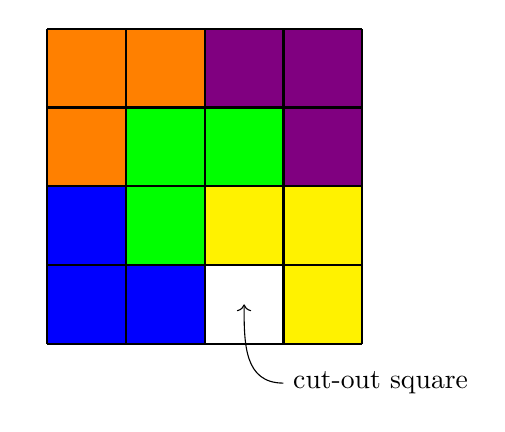
\begin{tikzpicture}
        \fill[blue] (0,0) rectangle (2,1);
        \fill[blue] (0,0) rectangle (1,2);
        \fill[orange] (0,4) rectangle (1,2);
        \fill[orange] (0,4) rectangle (2,3);
        \fill[violet] (4,4) rectangle (2,3);
        \fill[violet] (4,4) rectangle (3,2);
        \fill[green] (1,3) rectangle (2,1);
        \fill[green] (1,3) rectangle (3,2);
        \fill[yellow] (4,2) rectangle (2,1);
        \fill[yellow] (4,2) rectangle (3,0);
	  \foreach \x in {0,1,2,3,4}
	  {
	  \draw[thick] (0,\x) -- (4,\x);
	  \draw[thick] (\x,0) node[left]{} -- (\x,4);
	  }
        \draw [<-] (2.5,0.5) .. controls (2.5,0) and (2.5,-0.5) .. (3,-0.5) node[right]{cut-out square};
    \end{tikzpicture}
\end{center}


\answer  %%%% ANSWER TO PROBLEM 5 HERE %%%%
\\
We prove the statement by induction on $n \in \N$. It is easy to see that for $n=0$ we do not need to use any L-shaped tile, just leave the blank empty.

\textbf{Base Case ($n=1$):}
When $n=1$, the grid is a $2 \times 2$ square.
Removing any one square leaves exactly 3 squares, which can be perfectly covered by a single L-shaped tile.
Thus, the statement holds for $n=1$.

\textbf{Induction Step:}
Assume that for some $k \ge 1$, $n=k$, any $2^n \times 2^n$ grid with one square removed can be perfectly tiled by L-shaped tiles with no overlap.
We show that the statement holds for $n = k+1$.

Consider a $2^{k+1} \times 2^{k+1}$ grid with one square removed.
Divide the grid into four $2^k \times 2^k$ subgrids by drawing one vertical and one horizontal line through the center.
\begin{center}
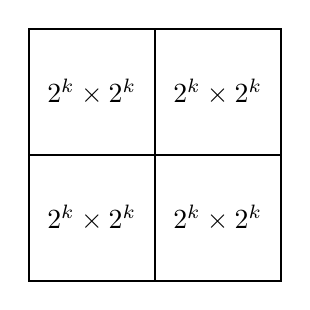
\begin{tikzpicture}[scale=0.8]

\draw[thick] (0,0) rectangle (4,4);

\draw[thick] (2,0) -- (2,4);
\draw[thick] (0,2) -- (4,2);

\node at (1,3) {$2^k \times 2^k$};
\node at (3,3) {$2^k \times 2^k$};
\node at (1,1) {$2^k \times 2^k$};
\node at (3,1) {$2^k \times 2^k$};

\end{tikzpicture}
\end{center}
By symmetry, exactly one of the four $2^k \times 2^k$ subgrids contains the missing square.\\
Without loss of generality, assume that the missing square lies in the bottom-right subgrid. Then we can use the result from $n=k$ to cover that subgrid.
\begin{center}
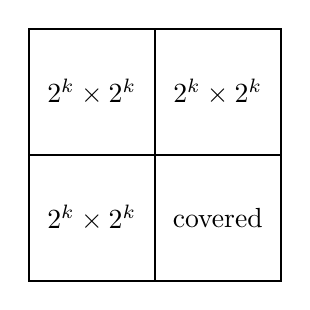
\begin{tikzpicture}[scale=0.8]
\draw[thick] (0,0) rectangle (4,4);
\draw[thick] (2,0) -- (2,4);
\draw[thick] (0,2) -- (4,2);

\node at (1,3) {$2^k \times 2^k$};
\node at (3,3) {$2^k \times 2^k$};
\node at (1,1) {$2^k \times 2^k$};

\node at (3,1) {covered};

\end{tikzpicture}
\end{center}
Place one L-shaped tile at the center of the grid (this case, I, II, and III quadrant) so that it covers one square from each of the other three subgrids.
After placing this tile, each of the four subgrids now has exactly one square missing.

\begin{center}
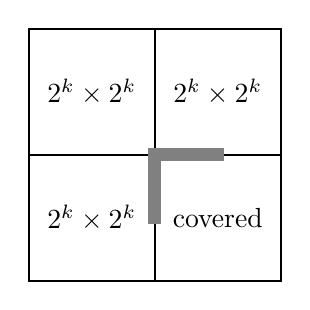
\begin{tikzpicture}[scale=0.8]

\draw[thick] (0,0) rectangle (4,4);

\draw[thick] (2,0) -- (2,4);
\draw[thick] (0,2) -- (4,2);


\fill[gray] (1.9,1.9) rectangle (2.1,2.1); 
\fill[gray] (1.9,0.9) rectangle (2.1,2.0);  
\fill[gray] (2.0,1.9) rectangle (3.1,2.1);  

\node at (1,3) {$2^k \times 2^k$};
\node at (3,3) {$2^k \times 2^k$};
\node at (1,1) {$2^k \times 2^k$};
\node at (3,1) {covered};

\end{tikzpicture}
\end{center}


By induction, each $2^k \times 2^k$ subgrid with one square removed can be perfectly tiled by L-shaped tiles.
Therefore, the entire $2^{k+1} \times 2^{k+1}$ grid can be tiled with no overlap.

\textbf{Conclusion:}
By mathematical induction, for all $n \in \N$, any $2^n \times 2^n$ grid with one square removed can be perfectly covered by L-shaped tiles.
\qed







\newpage
\problem Determine if each statement below is always, sometimes, or never true. If a statement is sometimes true, give a brief explanation of what conditions make it true.

\begin{enumerate}[(a)]
    \item Let $x,y$ be arbitrary objects. Then $\{x,y\} = \{y,x\}$.
    \item Let $x,y$ be arbitrary objects. Then $(x,y) = (y,x)$.
    \item Let $X$  be a set. Then $\{ \emptyset, X\} \subseteq \mathscr{P}(X)$.
    \item Let $X$ be a set and let $A \subseteq X$. Then $A \in X$.
    \item Let $X,Y,Z$ be sets. Then $(X \times Y) \times Z = X \times (Y \times Z)$.
\end{enumerate}

\answer  %%%% ANSWER TO PROBLEM 6 HERE %%%%
\begin{enumerate}[(a)]
    \item Always true.
    \item Sometimes true. When $x=y$, $(x,y) = (x, x)=(y,x)$.
    \item Always true.
    \item Sometimes true. True case, if $A = \emptyset$, let X be the $\mathscr{P}(\{1, 2\})$, then $A \subseteq X$ and $A \in X$. False case, let $A= \{1\}$ and $X= \{1,2\}$, $A \subseteq X$ but $A \notin X$. 
    \item Sometimes true. If one of the sets is the empty set, then both sides are empty sets. However, generally, this statement is not true.
\end{enumerate}






\end{document}